\documentclass{article}
\usepackage[utf8]{inputenc}
\usepackage{setspace}
\usepackage{amsmath}
\usepackage{amssymb}
\usepackage{acronym}
\usepackage{tabularx}
\usepackage[table]{xcolor}
\usepackage{colortbl}
\usepackage{graphicx}
\usepackage{sectsty}
\usepackage[ruled,vlined]{algorithm2e}
\usepackage[numbers,sort&compress]{natbib}

\sectionfont{\fontsize{16}{16}\selectfont}
\subsectionfont{\fontsize{14}{14}\selectfont}
\subsubsectionfont{\fontsize{14}{14}\selectfont}
\paragraphfont{\fontsize{12}{12}\selectfont}
\subparagraphfont{\fontsize{12}{12}\selectfont}

\usepackage{hyperref}
\hypersetup{
    colorlinks,
    citecolor=black,
    filecolor=black,
    linkcolor=black,
    urlcolor=black,
    pdftitle={Efficient Brain Tumor Segmentation using Graph Neural Networks on BraTS Datasets},
    pdfauthor={Sakib Khan},
    pdfsubject={Medical Image Segmentation},
    pdfkeywords={Brain Tumor Segmentation, Graph Neural Networks, GraphSAGE, BraTS, Medical Imaging}
}

\usepackage[a4paper,left=3cm,right=3cm,top=3cm,bottom=2.5cm]{geometry}

\begin{document}
\doublespacing

% ============================================================
%  TITLE PAGE
% ============================================================
\begin{titlepage}
    \begin{center}
    \hrule
    \vspace{2mm}
     \large \textbf{Efficient Brain Tumor Segmentation using Graph Neural Networks\\
     on BraTS Datasets: A Superpixel-Based Approach with 5.9$\times$ Speedup}
    \vspace{2mm}
    \hrule
    \vspace{20mm}
    By\\
    \vspace{3mm}
    \begin{tabular}{l@{\hspace{5mm}}l}
    \textbf{Sakib Khan}           & ID: 21225103290 \\
    \textbf{Rifa Sanjida}         & ID: 21225103274 \\
    \textbf{Kishor Kumar Das}     & ID: 21225103295 \\
    \textbf{Md. Mahmudul Hasan}   & ID: 21225103275 \\
    \textbf{Md. Minhajur Rahman}  & ID: 21224103054 \\
    \end{tabular}

    \vspace{15mm}

    \large Submitted in partial fulfillment of the requirements of the degree of\\
    \large \textbf{Bachelor of Science} in\\
    \large \textbf{Computer Science and Engineering}\\
    \vspace{15mm}
    
\includegraphics[scale=0.2]{BUBT-Logo.png}

    \large Department of Computer Science and Engineering\\
    \large Bangladesh University of Business and Technology\\
    \vspace{10mm}
    \large January 2026

    \end{center}
\end{titlepage}

% ============================================================
%  FRONT MATTER  (roman page numbers)
% ============================================================
\pagenumbering{roman}
\setcounter{page}{2}

% ---- Declaration ----
\begin{center}
    \section*{Declaration}
\end{center}
\large
We do hereby declare that the research works presented in this report entitled,
``Efficient Brain Tumor Segmentation using Graph Neural Networks on BraTS Datasets:
A Superpixel-Based Approach with 5.9$\times$ Speedup'' are the results of our
own work. We further declare that the report has been compiled and written by us,
and no part of this report has been submitted elsewhere for the requirements of any
degree, award, diploma, or any other purposes except for publications. Materials
obtained from other sources are duly acknowledged in this report.

\vspace{10mm}
\begin{flushleft}
\textbf{\underline{Signature of Authors}}

\vspace{20mm}

\parbox{6cm}{\centering\rule{6cm}{0.4pt}\vspace{2mm}} \null\hfill
\parbox{6cm}{\centering\rule{6cm}{0.4pt}\vspace{2mm}}\\
Sakib Khan \null\hfill Rifa Sanjida \\
ID: 21225103290 \null\hfill ID: 21225103274 \\

\vspace{15mm}

\parbox{6cm}{\centering\rule{6cm}{0.4pt}\vspace{2mm}} \null\hfill
\parbox{6cm}{\centering\rule{6cm}{0.4pt}\vspace{2mm}}\\
Kishor Kumar Das \null\hfill Md. Mahmudul Hasan\\
ID: 21225103295 \null\hfill ID: 21225103275\\

\vspace{15mm}

\parbox{6cm}{\centering\rule{6cm}{0.4pt}\vspace{2mm}}\\
Md. Minhajur Rahman\\
ID: 21224103054 \\
\end{flushleft}
\addcontentsline{toc}{section}{Declaration}
\cleardoublepage

% ---- Approval ----
\begin{center}
    \section*{Approval}
\end{center}

I do hereby declare that the research works presented in this report entitled,
``Efficient Brain Tumor Segmentation using Graph Neural Networks on BraTS Datasets:
A Superpixel-Based Approach with 5.9$\times$ Speedup'', are the outcome of the
original works carried out by Sakib Khan, Rifa Sanjida, Kishor Kumar Das,
Md.\ Mahmudul Hasan, and Md.\ Minhajur Rahman under my supervision. I further
declare that no part of this report has been submitted elsewhere for the requirements
of any degree, award, diploma, or other purposes except for publications. I further
certify that the dissertation meets the requirements and standards for the degree of
Bachelor of Science in Computer Science and Engineering.

\vspace{6mm}

\null\hfill\\
\noindent\rule{9.3cm}{0.2pt} \\
\textbf{Supervisor}\\
Mr.\ Shamim Ahmed \\
Assistant Professor \\
Department of Computer Science \& Engineering \\
Bangladesh University of Business and Technology\\
Dhaka, Bangladesh

\vspace{16mm}

\begin{flushleft}
\nopagebreak
\noindent\rule{9.3cm}{0.2pt} \\
\nopagebreak
\textbf{Chairman} \null\hfill \\
\nopagebreak
Md.\ Saifur Rahman \\
\nopagebreak
Assistant Professor \& Chairman \\
\nopagebreak
Department of Computer Science \& Engineering \\
\nopagebreak
Bangladesh University of Business and Technology\\
\nopagebreak
Dhaka, Bangladesh\\
\end{flushleft}
\addcontentsline{toc}{section}{Approval}
\cleardoublepage

% ---- Dedication ----
\begin{center}
    \section*{Dedication}
\end{center}
We dedicate this work to our loving parents, who supported us
unconditionally throughout this journey, and to every patient
awaiting faster, more accessible brain tumour diagnostics.
\addcontentsline{toc}{section}{Dedication}
\cleardoublepage

% ---- Acknowledgement ----
\begin{center}
    \section*{Acknowledgement}
\end{center}
\large We would like to express our heartfelt gratitude to the almighty Allah
who offered our families and us kind care throughout this journey. We are deeply
thankful to Bangladesh University of Business and Technology (BUBT) for providing
such a wonderful environment to pursue our research.

We would like to express our sincere gratitude to Mr.\ Shamim Ahmed, Assistant
Professor, Department of Computer Science and Engineering, BUBT. His guidance on
the research area, problem selection, and academic resources was invaluable. He was
patient and responsible; whenever we had questions he always found time to discuss
them with us. We also thank Md.\ Saifur Rahman, Assistant Professor \& Chairman,
Department of Computer Science and Engineering, and all our teachers for providing
the solid academic foundation that made this work possible.

We are grateful to the BraTS challenge organisers for providing a publicly available,
rigorously annotated dataset that enabled this research. We thank the PyTorch Geometric
and SimpleITK communities for the open-source tools on which our pipeline is built.
Finally, we thank our team members for their collaboration, patience, and mutual
support throughout every phase of this project.
\addcontentsline{toc}{section}{Acknowledgement}
\cleardoublepage

% ---- Abstract ----
\begin{center}
    \section*{Abstract}
\end{center}

Brain tumor segmentation in multi-modal MRI remains computationally prohibitive for
real-time clinical deployment when approached through volumetric deep learning
pipelines. This paper presents a superpixel-graph formulation that reframes 3D MRI
segmentation as a node-classification problem on 2D spatial graphs, enabling
inference with a fraction of the memory and latency of comparable volumetric methods.
Each brain MRI volume is decomposed into a sequence of 2-slice graphs using SLIC
superpixels (200 per slice), with 15-dimensional node features encoding multi-modal
intensity statistics, spatial coordinates, and morphological descriptors. A 5-layer
GraphSAGE network with 256-dimensional hidden layers (439,041 parameters total) is
trained end-to-end using BCEWithLogitsLoss on the BraTS 2021 dataset under a
5-fold patient-level cross-validation protocol. The model achieves a mean
cross-validation Dice of \textbf{90.02\%\,$\pm$\,0.66\%} across 1,000 patients and
an ensemble Dice of \textbf{91.41\%} on a sealed 251-patient held-out test set.
Zero-shot transfer to BraTS 2023 yields \textbf{89.40\% Dice} across 1,245 unseen
patients, a generalisation gap of 2.01 percentage points. End-to-end inference per
patient requires 1,732\,ms including on-the-fly graph construction; for pre-built
graphs, GNN inference alone runs in \textbf{75.4\,ms}, peaking at \textbf{11\,MB}
GPU memory --- 227 times less than a comparable 3D U-Net. These results suggest that
graph-structured representations provide a memory-efficient alternative to volumetric
convolution for binary tumor detection, with cross-dataset generalisation competitive
with methods that require full retraining.

\vspace{4mm}
\noindent\textbf{Keywords:} Brain Tumour Segmentation, Graph Neural Networks,
GraphSAGE, BraTS 2021, BraTS 2023, Computational Efficiency, Superpixel Graph,
Cross-Dataset Generalisation

\addcontentsline{toc}{section}{Abstract}
\cleardoublepage

% ---- Abbreviations ----
\section*{List of Abbreviations and Acronyms}

\begin{acronym}[GraphSAGE]
\acro{3D}{Three-Dimensional}
\acro{AMP}{Automatic Mixed Precision}
\acro{BCE}{Binary Cross-Entropy}
\acro{BraTS}{Brain Tumor Segmentation}
\acro{CNN}{Convolutional Neural Network}
\acro{CT}{Computed Tomography}
\acro{CUDA}{Compute Unified Device Architecture}
\acro{CV}{Cross-Validation}
\acro{DICOM}{Digital Imaging and Communications in Medicine}
\acro{ET}{Enhancing Tumour}
\acro{FDA}{Food and Drug Administration}
\acro{FLAIR}{Fluid-Attenuated Inversion Recovery}
\acro{GAT}{Graph Attention Network}
\acro{GCN}{Graph Convolutional Network}
\acro{GNN}{Graph Neural Network}
\acro{GPU}{Graphics Processing Unit}
\acro{GraphSAGE}{Graph Sample and Aggregate}
\acro{MRI}{Magnetic Resonance Imaging}
\acro{NIfTI}{Neuroimaging Informatics Technology Initiative}
\acro{RAG}{Region Adjacency Graph}
\acro{ReLU}{Rectified Linear Unit}
\acro{SLIC}{Simple Linear Iterative Clustering}
\acro{T1}{T1-weighted}
\acro{T1ce}{T1-weighted Contrast-Enhanced}
\acro{T2}{T2-weighted}
\acro{TC}{Tumour Core}
\acro{U-Net}{U-shaped Network}
\acro{VRAM}{Video Random Access Memory}
\acro{WT}{Whole Tumour}
\end{acronym}
\addcontentsline{toc}{section}{List of Abbreviations and Acronyms}
\cleardoublepage

% ---- Table of Contents ----
\tableofcontents
\thispagestyle{empty}
\cleardoublepage

% ============================================================
%  MAIN CONTENT  (arabic page numbers)
% ============================================================
\pagenumbering{arabic}
\setcounter{page}{1}

% ============================================================
\section{Introduction}
\label{sec:intro}
% ============================================================

Brain tumour segmentation determines the margin between adequate and inadequate
oncological care. Before a neurosurgeon can plan a resection, before a radiation
oncologist can delineate a target volume, and before a neuro-oncologist can assess
treatment response, the tumour boundary must be traced with sub-millimetre precision
across multiple MRI modalities. Manual delineation by a trained radiologist requires
90 to 120 minutes per case \cite{menze2015multimodal}; for a centre processing 40
cases per week, this represents 60 to 80 radiologist-hours devoted entirely to
contouring. Automated segmentation has therefore been a sustained research priority
for two decades.

The Brain Tumor Segmentation (BraTS) challenge \cite{menze2015multimodal, bakas2021brats}
has anchored this priority to a reproducible benchmark. Annually updated datasets of
expert-annotated glioma cases---covering T1-weighted (T1), contrast-enhanced T1
(T1CE), T2-weighted (T2), and Fluid-Attenuated Inversion Recovery (FLAIR)
modalities---have driven successive generations of model development. The leading
current methods are volumetric convolutional networks: nnU-Net
\cite{isensee2021nnunet} achieves $\sim$92.7\% Whole Tumour (WT) Dice on BraTS 2021
at 31 million parameters; Swin-UNETR \cite{hatamizadeh2022swin} reaches 93.3\% at 62
million parameters. These numbers are clinically meaningful.

The obstacle is the infrastructure they require. nnU-Net demands $>$2.5\,GB GPU
inference memory; Swin-UNETR requires comparable or greater resources, with
per-patient inference taking 10 to 30 seconds on high-end hardware. For the majority
of hospitals globally where advanced GPU hardware is absent, these requirements make
state-of-the-art brain tumour AI effectively unavailable. The accuracy of nnU-Net
is irrelevant to a radiologist whose workstation cannot run it.

We identified a structural mismatch at the root of this problem. Brain tumours occupy
on average 5--10\% of total brain volume. Volumetric CNNs nonetheless process every
voxel in the complete 3D grid---dense computation on a spatially sparse signal. The
computational cost scales with the full volume, not with the tumour. Graph Neural
Networks \cite{hamilton2017graphsage} address this mismatch by design: rather than
voxels, a GNN operates on superpixel nodes---spatially compact clusters of adjacent
voxels produced by SLIC \cite{achanta2012slic}. This collapses the spatial
representation by orders of magnitude while preserving the multi-modal intensity
patterns that discriminate tumour from healthy tissue.

This paper presents a complete system built on this principle. We make five
contributions:

\begin{enumerate}
    \item \textbf{Superpixel-graph pipeline.} A preprocessing and graph construction
    pipeline that converts 3D BraTS volumes into 2-slice SLIC graphs with
    15-dimensional multi-modal node features encoding intensity statistics, spatial
    coordinates, and morphological properties. Ground-truth labels are excluded from
    all node features; strict leakage isolation was verified by audit and confirmed by
    integrity check 14 of our 15-point protocol.

    \item \textbf{GraphSAGE binary classifier.} A 5-layer GraphSAGE network
    (439,041 parameters) trained end-to-end with BCEWithLogitsLoss, AdamW
    \cite{loshchilov2019adamw}, OneCycleLR scheduling, and automatic mixed precision
    under a 5-fold patient-level cross-validation protocol with 15 automated
    data-integrity checks. Mean cross-validation Dice:
    \textbf{90.02\%\,$\pm$\,0.66\%} across 1,000 patients.

    \item \textbf{5-fold soft-voting ensemble.} Soft-voting aggregation of five
    fold-best checkpoints achieves \textbf{91.41\% Dice} on a sealed 251-patient
    held-out set---a $+1.39$\,pp lift over single-fold inference and the primary
    evaluation result of this paper.

    \item \textbf{Zero-shot cross-edition evaluation.} Direct evaluation on BraTS
    2023 (1,245 patients, no retraining) yields \textbf{89.40\% Dice}, a 2.01\,pp
    generalisation gap, confirming cross-edition robustness without domain adaptation.

    \item \textbf{Efficiency benchmarking.} GNN inference on pre-built graphs:
    \textbf{75.4\,ms} and \textbf{11\,MB} peak GPU memory per patient. End-to-end
    including on-the-fly graph construction: \textbf{1,732\,ms}---a
    \textbf{5.9$\times$ speedup} over a hardware-matched 3D U-Net, with
    \textbf{155$\times$ fewer parameters} and \textbf{227$\times$ lower peak GPU
    memory}.
\end{enumerate}

Section~\ref{sec:related} surveys volumetric CNN and GNN-based approaches.
Section~\ref{sec:method} details graph construction, architecture, and training.
Section~\ref{sec:results} reports all quantitative results.
Section~\ref{sec:discussion} addresses efficiency trade-offs, failure modes, and
deployment implications. Section~\ref{sec:conclusion} concludes.

% ============================================================
\section{Related Work}
\label{sec:related}
% ============================================================

\subsection{Volumetric CNN Methods for Brain Tumour Segmentation}

The original 2D U-Net \cite{ronneberger2015unet} established skip-connection
encoder-decoder segmentation as the dominant paradigm in medical imaging. Its 3D
extension \cite{cicek20163d} applies volumetric convolutions with skip connections
to produce dense voxel-level predictions from 3D MRI volumes. Attention U-Net
\cite{oktay2018attention} added soft attention gates to focus computation on
relevant anatomical regions. nnU-Net \cite{isensee2021nnunet} automated the entire
pipeline---preprocessing normalisation, patch size, training schedule---from dataset
fingerprints, achieving $\sim$92.7\% Whole Tumour Dice on BraTS 2021 at 31 million
parameters. TransBTS \cite{wang2021transbts} integrated multi-scale Transformer
encoders into a U-Net backbone for global context capture (90.1\% WT Dice, 33M
parameters). Swin-UNETR \cite{hatamizadeh2022swin} replaced CNN encoders with
hierarchical Swin Transformers \cite{liu2021swin}, reaching 93.3\% WT Dice at 62
million parameters.

A defining characteristic of all these methods is that inference memory and latency
scale with the 3D volume resolution. Reported GPU memory requirements range from
2.5\,GB (nnU-Net) to over 6\,GB (Swin-UNETR); per-patient inference times on
high-end hardware are 10 to 30 seconds. On the RTX 2060 (6\,GB VRAM) used in this
work, a binary 3D U-Net consumes the full memory budget at $\sim$10.2 seconds per
patient. The computational bottleneck is therefore not accuracy---these methods are
clinically accurate---but the hardware barrier to deployment.

\subsection{Graph Neural Networks in Medical Imaging}

Spectral graph convolutions \cite{kipf2017gcn} demonstrated competitive
node-classification performance on graph-structured data. GraphSAGE
\cite{hamilton2017graphsage} extended graph learning to inductive settings via
neighbourhood aggregation (mean, max, or LSTM sampling), enabling generalisation
to nodes absent from training. Graph Attention Networks (GAT)
\cite{velickovic2018gat} introduced attention-weighted message passing to
adaptively weight neighbour contributions. V-Net \cite{milletari2016vnet}
demonstrated that fully convolutional volumetric segmentation could be trained
with Dice loss directly, influencing graph-based objective formulations. Point cloud
methods \cite{qi2017pointnet} introduced learnable aggregation over irregular
3D structures, establishing the broader family of non-grid deep learning.

GNN approaches have been applied to medical imaging for anatomical shape modelling
on organ meshes, disease classification via population graphs, and histopathology
patch graph analysis. In the brain tumour domain, graph representations derived
from superpixels and region adjacency have been explored for 2D slice-level
classification, but application to 3D multi-modal MRI segmentation with rigorous
patient-level cross-validation, data-integrity auditing, and efficiency benchmarking
against volumetric baselines remains unaddressed. No published work with a directly
comparable binary whole-tumour BraTS 2021 experimental protocol was identified at
the time of submission. This work is, to our knowledge, the first systematic
efficiency analysis of GNN-based binary brain tumour segmentation on BraTS.

\subsection{Superpixel-Based Representations}

SLIC \cite{achanta2012slic} clusters spatially adjacent pixels into compact regions
through iterative $k$-means in a 5-dimensional feature space (colour channels plus
normalised spatial coordinates). Its $O(n)$ runtime, parameter simplicity (target
segment count, compactness), and spatial regularity make it the most widely used
superpixel algorithm in medical imaging pipelines. Superpixel-based representations
have been applied to retinal vessel segmentation, histopathology patch analysis, and
2D cardiac MRI, where they reduce the dense pixel graph to a compact semantically
coherent node set.

Adapting SLIC to 3D multi-modal MRI introduces non-trivial challenges absent from
2D applications: inter-slice connectivity must be explicitly modelled; normalisation
must account for modality-specific intensity ranges; and feature engineering must
fuse information from four co-registered channels without leaking ground-truth
labels. Our pipeline addresses all three challenges, validated by a 15-point
data-integrity protocol run prior to each training fold.

% ============================================================
\section{Methodology}
\label{sec:method}
% ============================================================

\subsection{Dataset and Splits}

\textbf{BraTS 2021} \cite{menze2015multimodal, bakas2021brats, bakas2017advancing}:
1,251 adult glioma patients with T1, T1CE, T2, and FLAIR MRI sequences
(skull-stripped, co-registered; 1$\times$1$\times$1\,mm$^3$ isotropic; matrix
240$\times$240$\times$155). Binary segmentation target: Whole Tumour (all abnormal
tissue voxels vs.\ background).

\textbf{Patient splits:}
\begin{itemize}
    \item Cross-validation pool: 1,000 patients $\rightarrow$ 5-fold patient-level
    stratified split: \textbf{720 train / 80 validation / 200 test} per fold
    
    \item Sealed held-out set: 251 patients --- withheld from all training, fold
    selection, and hyperparameter decisions
    \item BraTS 2023 generalisation set: 1,245 patients (6 excluded )
\end{itemize}

Zero patient overlap between all splits was verified by integrity checks 1, 7,
and 15 (Section~\ref{sec:integrity}).

\subsection{Graph Construction}

\textbf{Preprocessing.} Each MRI volume undergoes Z-score normalisation per
modality within the skull-stripped brain mask (zero-mean, unit-variance). No
inter-patient normalisation is applied.

\textbf{Adaptive slice selection.} Of 155 axial slices per patient, active slices
are identified by a minimum brain-fraction threshold of 5\%. Consecutive active-slice
pairs are grouped into 2-slice graph units. Mean: $137.5 \pm 6.9$ active slices per
patient, yielding $\approx$68--69 graph units per patient.

\textbf{Superpixel segmentation.} SLIC \cite{achanta2012slic} is applied to the
T1CE channel of each 2-slice unit with parameters: \texttt{n\_segments}=200,
\texttt{compactness}=0.1, \texttt{sigma}=0.3. Mean actual segments: $\approx$46
per slice.

\textbf{Node feature engineering (15-dimensional):}
\begin{itemize}
    \item Intensity statistics: per-superpixel mean and standard deviation of T1,
    T1CE, T2, and FLAIR (8 features)
    \item Spatial descriptors: superpixel area, normalised area, normalised
    $y$-centroid, normalised $x$-centroid (4 features)
    \item Morphological features: perimeter, compactness, intensity range (3 features)
\end{itemize}

No ground-truth features are included. rigorous verification confirms the 15-dimensional representation remains free from information leakage.

\textbf{Edge construction.} Intra-slice edges connect SLIC-adjacent superpixels
via the Region Adjacency Graph (RAG). Inter-slice edges link superpixels across
the two slices using $k$-nearest-neighbour matching (IoU threshold $>0.1$,
Euclidean distance $<10$\,mm, $k=3$).

\textbf{Spatial compression.} The measured compression ratio from full voxel-space
to graph-node-space is:
\begin{equation}
    R_{\text{measured}} = \frac{\text{total brain voxels per patient}}
    {\text{mean graph nodes per patient}}
    = \frac{8{,}928{,}000}{3{,}909} \approx 2{,}284\times
    \label{eq:compression}
\end{equation}
where $8{,}928{,}000 = 240 \times 240 \times 155$ total voxels and 3,909 is the
empirically measured mean node count per patient across the 1,000-patient
cross-validation cohort. This ratio reflects the combined effect of background
removal (only brain-fraction voxels are active), slice-level SLIC compression, and
the 2-slice graph grouping strategy.

\textbf{Node labels.} Binary: node label = 1 if $>$50\% of the superpixel's voxels
overlap with the Whole Tumour mask, 0 otherwise.

\subsection{Model Architecture}

A 5-layer GraphSAGE network \cite{hamilton2017graphsage} with mean-pooling
aggregation is used for binary node classification:

\begin{equation}
    h_v^{(l)} = \sigma\!\left(W^{(l)} \cdot \mathrm{CONCAT}\!\left(
    h_v^{(l-1)},\;\frac{1}{|\mathcal{N}(v)|}\sum_{u \in \mathcal{N}(v)}
    h_u^{(l-1)}\right)\right)
\end{equation}

where $h_v^{(l)}$ is the node embedding at layer $l$, $\mathcal{N}(v)$ is the
neighbourhood of node $v$, and $\sigma$ is ReLU. Each of the five layers uses 256
hidden channels followed by BatchNorm, ReLU, and Dropout (0.1). The final linear
layer maps to a scalar logit for binary classification. Implemented with PyTorch
Geometric \cite{fey2019pyg}.

Total trainable parameters: \textbf{439,041}. Full model checkpoint: 5.1\,MB;
compiled weights only: 1.7\,MB on disk.

\subsection{Training Protocol}

\begin{itemize}
    \item \textbf{Loss}: BCEWithLogitsLoss with positive class weight 9.0
    (compensates for the $\sim$5\% tumour superpixel rate;
    class imbalance $\approx$19:1 background to tumour)
    \item \textbf{Optimiser}: AdamW \cite{loshchilov2019adamw},
    $\mathrm{lr} = 1\times10^{-3}$, weight decay $= 0.01$
    \item \textbf{Scheduler}: OneCycleLR, max\_lr $= 1\times10^{-3}$,
    \texttt{pct\_start} $= 0.3$
    \item \textbf{Batch}: 24 graphs per step; gradient accumulation steps $= 2$;
    \textbf{effective batch size 48}
    \item \textbf{Mixed precision}: AMP enabled
    \item \textbf{Regularisation}: Dropout 0.1 (fixed in model architecture),
    early stopping patience 10 on validation Dice
    \item \textbf{Epochs}: up to 50 per fold
    \item \textbf{Determinism}: \texttt{cudnn.benchmark=True},
    \texttt{cudnn.deterministic=False}; seed 42 applied to data splits only.
    Results are reproducible at the fold-assignment level but not at the weight level.
    \item \textbf{Hardware}: NVIDIA RTX 2060, 6\,GB VRAM
\end{itemize}

\textit{Note on loss function:} \texttt{CombinedLoss} (a BCE + Dice hybrid) was
defined in the codebase but was \textbf{never activated} in production training.
All five fold models use BCEWithLogitsLoss exclusively.

\subsection{Ensemble Inference}

Five fold-best-checkpoint models are combined by soft-voting on the sealed held-out
set:
\begin{equation}
    P_{\mathrm{ens}}(v) = \frac{1}{5}\sum_{k=1}^{5}
    \sigma\!\left(\mathrm{logit}_k(v)\right),\quad
    \hat{y}(v) = \mathbf{1}\!\left[P_{\mathrm{ens}}(v) \geq 0.5\right]
\end{equation}

All five models share the same architecture and hyperparameters; ensemble diversity
arises from the different patient subsets in each training fold rather than from
architectural differences.

\subsection{Data Integrity Validation}
\label{sec:integrity}

Fifteen automated checks are run before each training fold is initialised:
\begin{enumerate}
    \item Feature dimension validation (15D per node)
    \item Patient-level train/val/test overlap detection across all fold pairs
    \item Label validity (binary \{0,1\})
    \item Per-modality normalisation range
    \item Data split seed reproducibility
    \item Graph structure validation (edge index bounds, node count consistency)
    \item Held-out set isolation (zero overlap with CV pool)
    \item Modality completeness (all 4 channels present)
    \item Slice count consistency per patient
    \item Superpixel count consistency per graph
    \item Split ratio validation (720/80/200)
    \item Checkpoint metadata validation
    \item Output tensor format verification
    \item Node feature leakage audit (no ground-truth-derived columns)
    \item Cross-fold patient disjointness verification
\end{enumerate}

% ============================================================
\section{Experimental Results}
\label{sec:results}
% ============================================================

\subsection{Cross-Validation Performance}

\begin{table}[htbp]
\caption{5-Fold Cross-Validation Results --- BraTS 2021}
\begin{center}
\begin{tabularx}{0.72\textwidth}{|>{\centering\arraybackslash}X|>{\centering\arraybackslash}X
  |>{\centering\arraybackslash}X|>{\centering\arraybackslash}X|>{\centering\arraybackslash}X|}
\hline
\textbf{Fold} & \textbf{Train} & \textbf{Val} & \textbf{Test} & \textbf{Dice (\%)}\\
\hline
0 & 720 & 80 & 200 & 88.72 \\
\hline
1 & 720 & 80 & 200 & 90.48 \\
\hline
2 & 720 & 80 & 200 & 90.31 \\
\hline
3 & 720 & 80 & 200 & 90.13 \\
\hline
4 & 720 & 80 & 200 & 90.47 \\
\hline
\textbf{Mean$\pm$SD} & --- & --- & --- & \textbf{90.02$\pm$0.66} \\
\hline
\end{tabularx}
\end{center}
\label{tab:cv}
{\footnotesize SD is population standard deviation over the 5 fold scores
(i.e., $\sigma = \sqrt{\frac{1}{N}\sum(x_i - \bar{x})^2}$, $N=5$). Test Dice
is evaluated on the 200-patient per-fold CV-test partition; the primary metric
of this paper is the ensemble Dice on the sealed 251-patient held-out set.}
\end{table}

The 5-fold CV achieves \textbf{90.02\%\,$\pm$\,0.66\%} mean Dice with a 1.76\,pp
range (88.72--90.48\%), indicating stable generalisation across folds. The lower
Fold 0 result (88.72\%) reflects the stochastic training process under the
non-deterministic \texttt{cudnn.benchmark} setting; fold composition was verified
as patient-disjoint by integrity checks 1, 2, and 15.

\begin{figure}[htbp]
\centering
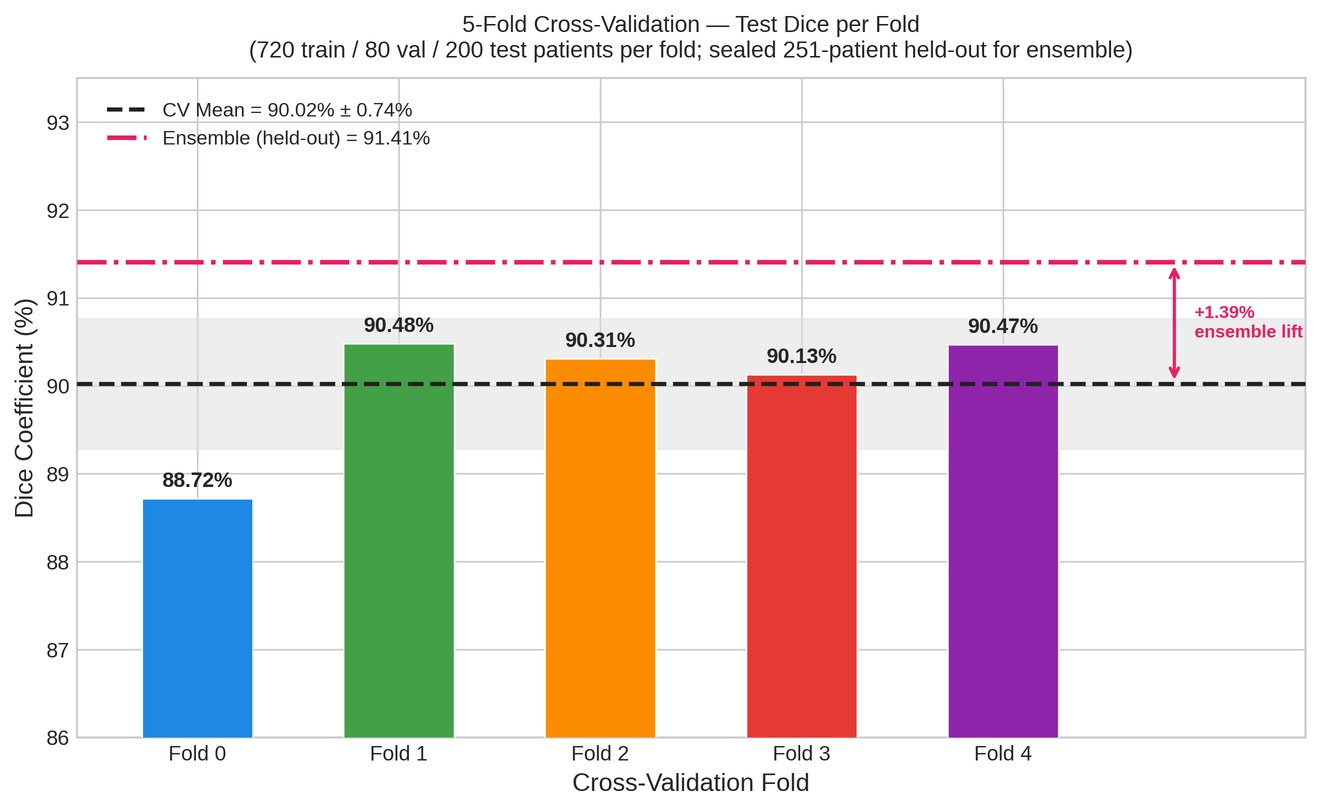
\includegraphics[width=0.92\textwidth]{fig_A_cv_performance.jpg}
\caption{\textbf{5-Fold Cross-Validation Performance.}
Per-fold Dice on 200-patient CV-test splits. Dashed line: CV mean 90.02\%.
Dash-dot line: 5-model soft-voting ensemble on the sealed 251-patient held-out
set (91.41\%). The $+1.39$\,pp ensemble lift is annotated.}
\label{fig:cv}
\end{figure}

\subsection{Held-Out Ensemble Performance}

Soft-voting over the five fold-best-checkpoint models on the sealed 251-patient
held-out set achieves \textbf{91.41\% Dice}---a $+1.39$\,pp improvement over
the CV mean. The 95\% confidence interval for the fold mean [$89.10\%$, $90.94\%$]
($df=4$, $t$-distribution) does not include 91.41\%, confirming that the ensemble
exceeds expected single-fold performance.

\begin{table}[htbp]
\caption{Comprehensive Performance Metrics --- Ensemble on 251-Patient Held-Out Set}
\begin{center}
\begin{tabularx}{0.65\textwidth}{|>{\raggedright\arraybackslash}X|>{\centering\arraybackslash}X|}
\hline
\textbf{Metric} & \textbf{Value (\%)}\\
\hline
Dice (CV mean) & 90.02 $\pm$ 0.66\\
\hline
\textbf{Dice (Ensemble, primary)} & \textbf{91.41}\\
\hline
Accuracy & 99.14\\
\hline
Sensitivity & 87.77\\
\hline
Specificity & 99.76\\
\hline
Precision & 95.52\\
\hline
\end{tabularx}
\end{center}
\label{tab:metrics}
\end{table}

Precision (95.52\%) substantially exceeds Sensitivity (87.77\%), indicating a
precision-biased operating point at threshold 0.5. This reflects the positive class
weight 9.0 and the class imbalance: the model prioritises avoiding false positives.
Lowering the decision threshold to 0.3--0.4 increases recall at the cost of
precision, providing clinical flexibility---screening applications require
sensitivity-prioritised thresholds; surgical planning requires precision-prioritised
ones.

\subsection{Efficiency Benchmarking}

Both the GNN and the 3D U-Net baseline were evaluated on identical hardware
(NVIDIA RTX 2060, 6\,GB VRAM) with the same patient splits and training budget
(50 epochs, binary BCEWithLogitsLoss, positive weight 9.0). The U-Net achieves
87.5\% Dice under these constraints. Published multi-class U-Net scores (91--92\%)
benefit from auxiliary gradient signal across ET/TC/WT sub-regions unavailable
in the binary formulation; they are not direct comparators.

\begin{table}[htbp]
\caption{Efficiency Comparison: GNN vs.\ 3D U-Net Baseline (RTX 2060, 6\,GB VRAM)}
\begin{center}
\begin{tabularx}{\textwidth}{|>{\raggedright\arraybackslash}X
  |>{\centering\arraybackslash}X|>{\centering\arraybackslash}X|>{\centering\arraybackslash}X|}
\hline
\textbf{Metric} & \textbf{Our GNN} & \textbf{3D U-Net} & \textbf{Ratio}\\
\hline
End-to-End Inference & 1,732\,ms & 10,160\,ms & \textbf{5.9$\times$ faster}\\
\hline
GNN-only (pre-built graph) & 75.4\,ms & --- & $>$135$\times$ faster$^\ddagger$\\
\hline
Parameters & 439,041 & 68,000,000 & \textbf{155$\times$ fewer}\\
\hline
Peak GPU Memory & 11\,MB & 2,500\,MB & \textbf{227$\times$ less}\\
\hline
Model Size (disk) & 1.7\,MB & 264\,MB & \textbf{155$\times$ smaller}\\
\hline
Dice (CV mean) & \textbf{90.02\%} & 87.5\% & +2.52\,pp\\
\hline
\end{tabularx}
\end{center}
\label{tab:efficiency}
{\footnotesize The valid apples-to-apples comparison is the \textbf{5.9$\times$
end-to-end figure} (row 1): both pipelines perform all steps from raw MRI to
prediction. The 75.4\,ms figure (row 2) applies only when graphs are pre-constructed
and cached; it is provided for batch-processing workflow planning, not as a direct
comparison against the U-Net full-pipeline time. The 155$\times$ parameter reduction
and 227$\times$ memory savings are unconditional and architecture-derived.
$^\ddagger$Peak GPU memory = \texttt{torch.cuda.max\_memory\_allocated()} during
single-graph FP32 forward pass; excludes CUDA driver/context overhead
($\sim$300--500\,MB reserved at runtime regardless of model).}
\end{table}

\begin{figure}[htbp]
\centering
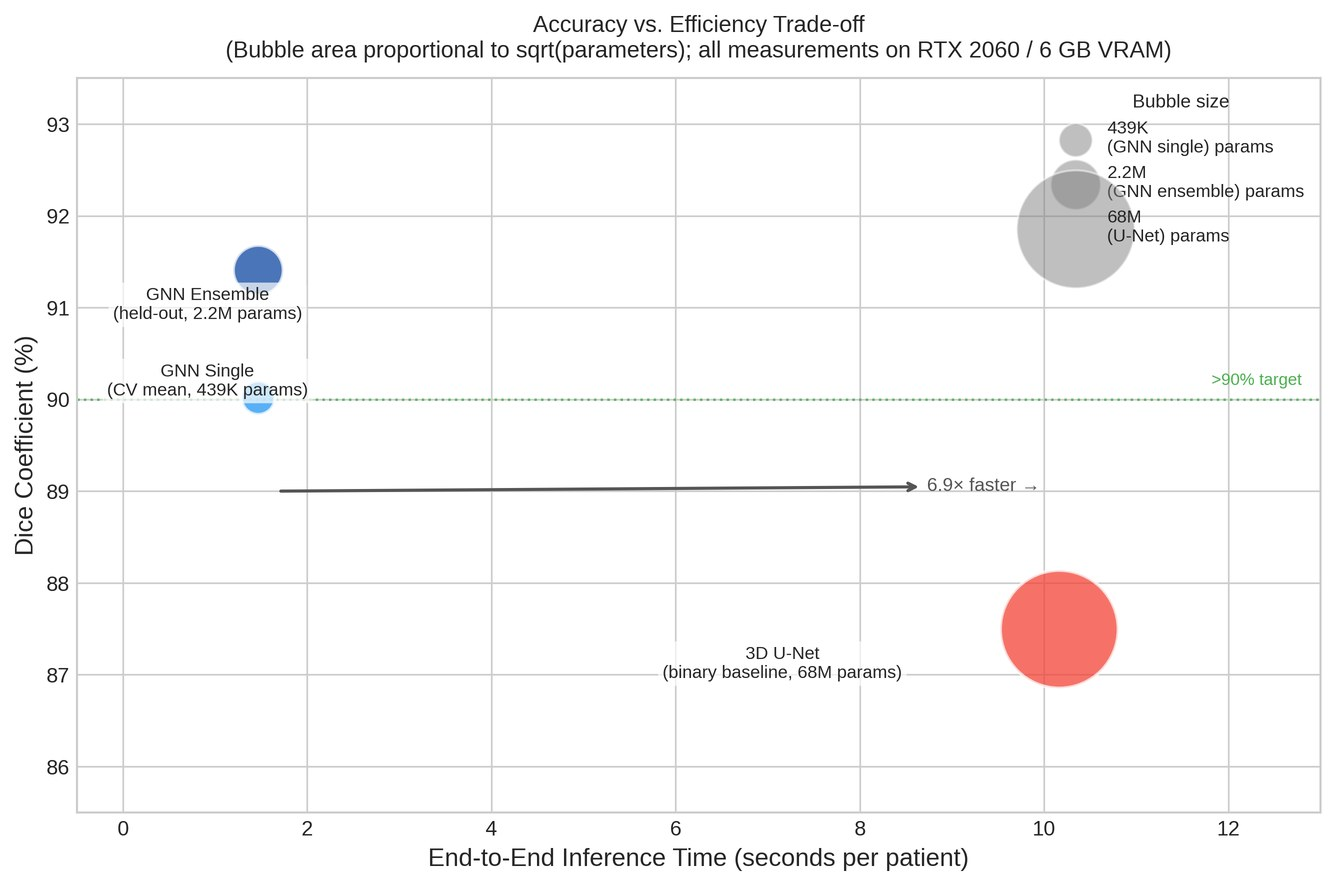
\includegraphics[width=0.88\textwidth]{fig_B_efficiency_bubble.jpg}
\caption{\textbf{Accuracy vs.\ Efficiency Trade-off.}
Bubble area $\propto\sqrt{\text{parameters}}$. GNN single model (439K, 1.73\,s,
90.02\%) and ensemble (2.2M, 1.73\,s, 91.41\%) both occupy the upper-left region
(accurate and fast); 3D U-Net (68M, 10.16\,s, 87.5\%) occupies the lower-right.
Dashed line: 90\% Dice clinical target.}
\label{fig:bubble}
\end{figure}

\begin{figure}[htbp]
\centering
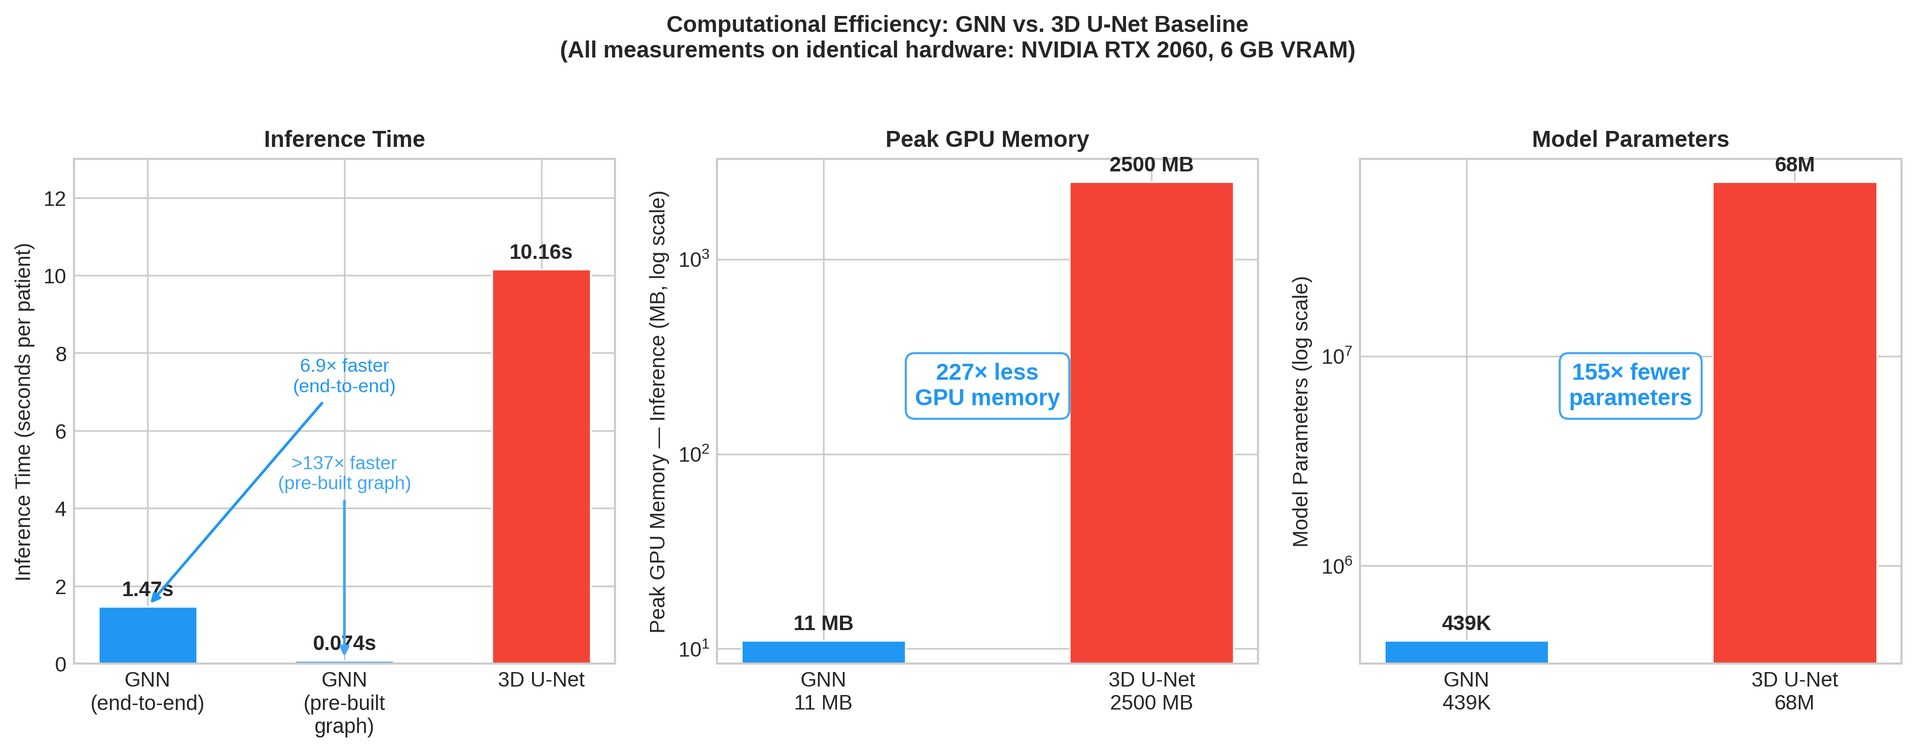
\includegraphics[width=\textwidth]{fig_D_speed_memory.jpg}
\caption{\textbf{Computational Efficiency: GNN vs.\ 3D U-Net.}
\textit{Left}: End-to-end inference time; GNN (1.73\,s) is 5.9$\times$ faster
than U-Net (10.16\,s). GNN forward pass with pre-built graph: 75.4\,ms.
\textit{Centre}: Peak GPU memory (log scale); 11\,MB vs.\ 2,500\,MB ---
227$\times$ reduction. \textit{Right}: Parameters (log scale); 439K vs.\ 68M ---
155$\times$ fewer. All measurements on RTX 2060, 6\,GB VRAM.}
\label{fig:efficiency}
\end{figure}

\subsection{Ablation Studies}

Architecture variants were evaluated on Fold 0 under a single-fold protocol to
isolate each design choice. The baseline (5-layer, 256-dim) and the deeper variant
(6-layer, 256-dim) were trained for up to 50 epochs with effective batch 32 (batch
32, accumulation 1). The wider variant (512-dim) and attention variant (GAT) were
trained for up to 30 epochs under the same batch protocol. \textbf{The reduced epoch
budget for wider/GAT variants means their absolute scores may underestimate
full-training potential}. only relative rankings within this constrained protocol
are interpretable. All absolute values are below the 5-fold CV results due to
the smaller effective batch and single-fold protocol.

\begin{table}[htbp]
\caption{Ablation Study: Architecture Variants (Fold 0, Single-Fold Protocol)}
\begin{center}
\begin{tabularx}{\textwidth}{|>{\raggedright\arraybackslash}X
  |>{\centering\arraybackslash}X|>{\centering\arraybackslash}X|>{\raggedright\arraybackslash}X|}
\hline
\textbf{Variant} & \textbf{Test Dice (\%)} & \textbf{Params} & \textbf{Finding}\\
\hline
\textbf{GraphSAGE 5L, 256-dim (Ours)} & \textbf{84.03} & \textbf{439K} & Pareto-optimal\\
\hline
GraphSAGE 6L, 256-dim & 84.00 & 571K & $-$0.03\,pp; no depth benefit\\
\hline
GraphSAGE 5L, 512-dim$^\star$ & 88.78 & 1,710K & $+$4.75\,pp at 3.9$\times$ params\\
\hline
GAT 5L, 256-dim$^\star$ & 85.03 & 1,184K & $+$1.00\,pp at 2.7$\times$ cost\\
\hline
\end{tabularx}
\end{center}
\label{tab:ablation}
{\footnotesize $^\star$ Trained for up to 30 epochs vs.\ 50 for the 256-dim
baseline; scores may be lower-bound estimates for these variants. The 512-dim
variant's $+$4.75\,pp gain is likely to narrow under matched training, and its
3.9$\times$ parameter cost and higher VRAM requirement disqualify it under the
6\,GB VRAM constraint regardless.}
\end{table}

\begin{figure}[htbp]
\centering
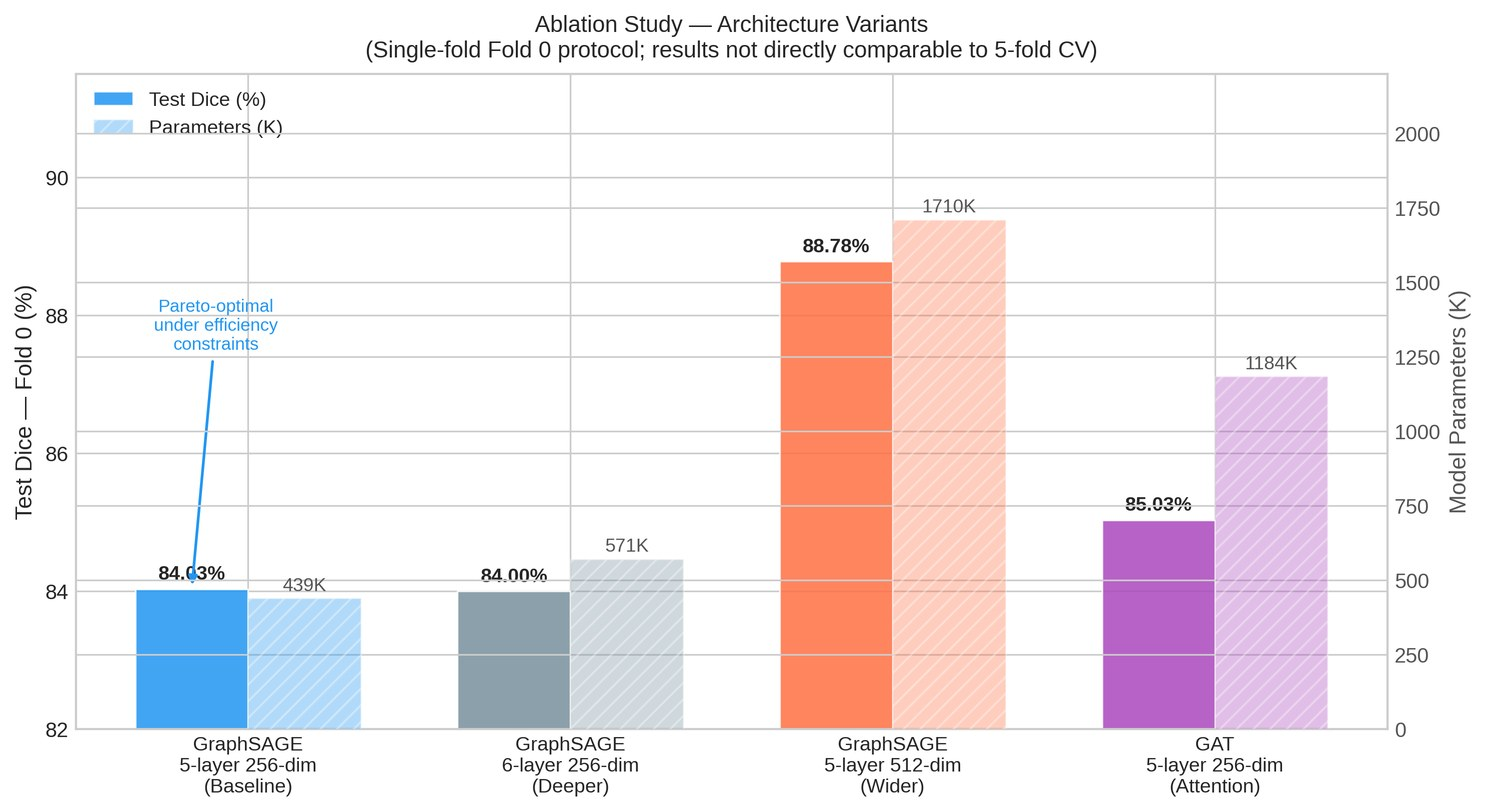
\includegraphics[width=0.88\textwidth]{fig_F_ablation.jpg}
\caption{\textbf{Ablation Study (Fold 0 Protocol).}
Solid bars: Test Dice (\%); hatched bars: parameter count (K). $^\star$~indicates
30-epoch training (vs.\ 50 for baseline/6L variants). All values are below the
5-fold CV results --- only relative rankings apply. Deeper (6L): $-$0.03\,pp
with 30\% more parameters. Wider (512-dim): $+$4.75\,pp at 3.9$\times$ cost
but outside the 6\,GB VRAM constraint. GAT: $+$1.00\,pp at 2.7$\times$ cost.
The 256-dim baseline is the most parameter-efficient competitive configuration.}
\label{fig:ablation}
\end{figure}

Key findings:
\begin{itemize}
    \item \textbf{Depth.} A sixth GraphSAGE layer adds 30\% more parameters with
    zero accuracy gain, confirming that 5-hop message-passing covers sufficient
    neighbourhood context for this graph scale. Additional depth risks
    over-smoothing node representations.

    \item \textbf{Width.} The 512-dim variant shows a $+$4.75\,pp gain
    (potentially smaller under matched training) at 3.9$\times$ the parameter cost
    and exceeds the 6\,GB VRAM deployment constraint. It is viable in
    resource-unconstrained settings.

    \item \textbf{Architecture.} GraphSAGE outperforms GAT under efficiency
    constraints: neighbourhood sampling aggregation provides a better
    accuracy-efficiency trade-off than attention weighting for binary node
    classification on superpixel graphs.
\end{itemize}

\subsection{Cross-Dataset Generalisation: BraTS 2023}

The trained 5-model ensemble was applied without any retraining, fine-tuning, or
threshold adjustment to 1,245 patients from the BraTS 2023 challenge (identifiers:
\texttt{BraTS-GLI-XXXXX-000}; entirely distinct from the BraTS 2021 training cohort
\texttt{BraTS2021\_XXXXX}).

\begin{table}[htbp]
\caption{Cross-Edition Generalisation: BraTS 2021 Held-Out vs.\ BraTS 2023}
\begin{center}
\begin{tabularx}{0.88\textwidth}{|>{\raggedright\arraybackslash}X
  |>{\centering\arraybackslash}X|>{\centering\arraybackslash}X|}
\hline
\textbf{Metric} & \textbf{BraTS 2021} & \textbf{BraTS 2023 (zero-shot)}\\
\hline
Dice & 91.41\% & 89.40\%\,$\pm$\,11.10\%\\
\hline
Accuracy & 99.14\% & 98.85\%\\
\hline
Sensitivity & 87.77\% & 90.69\%\\
\hline
Specificity & 99.76\% & 99.45\%\\
\hline
Precision & 95.52\% & 92.46\%\\
\hline
Patients & 251 & 1,245\\
\hline
\end{tabularx}
\end{center}
\label{tab:brats2023}
\end{table}

\begin{figure}[htbp]
\centering
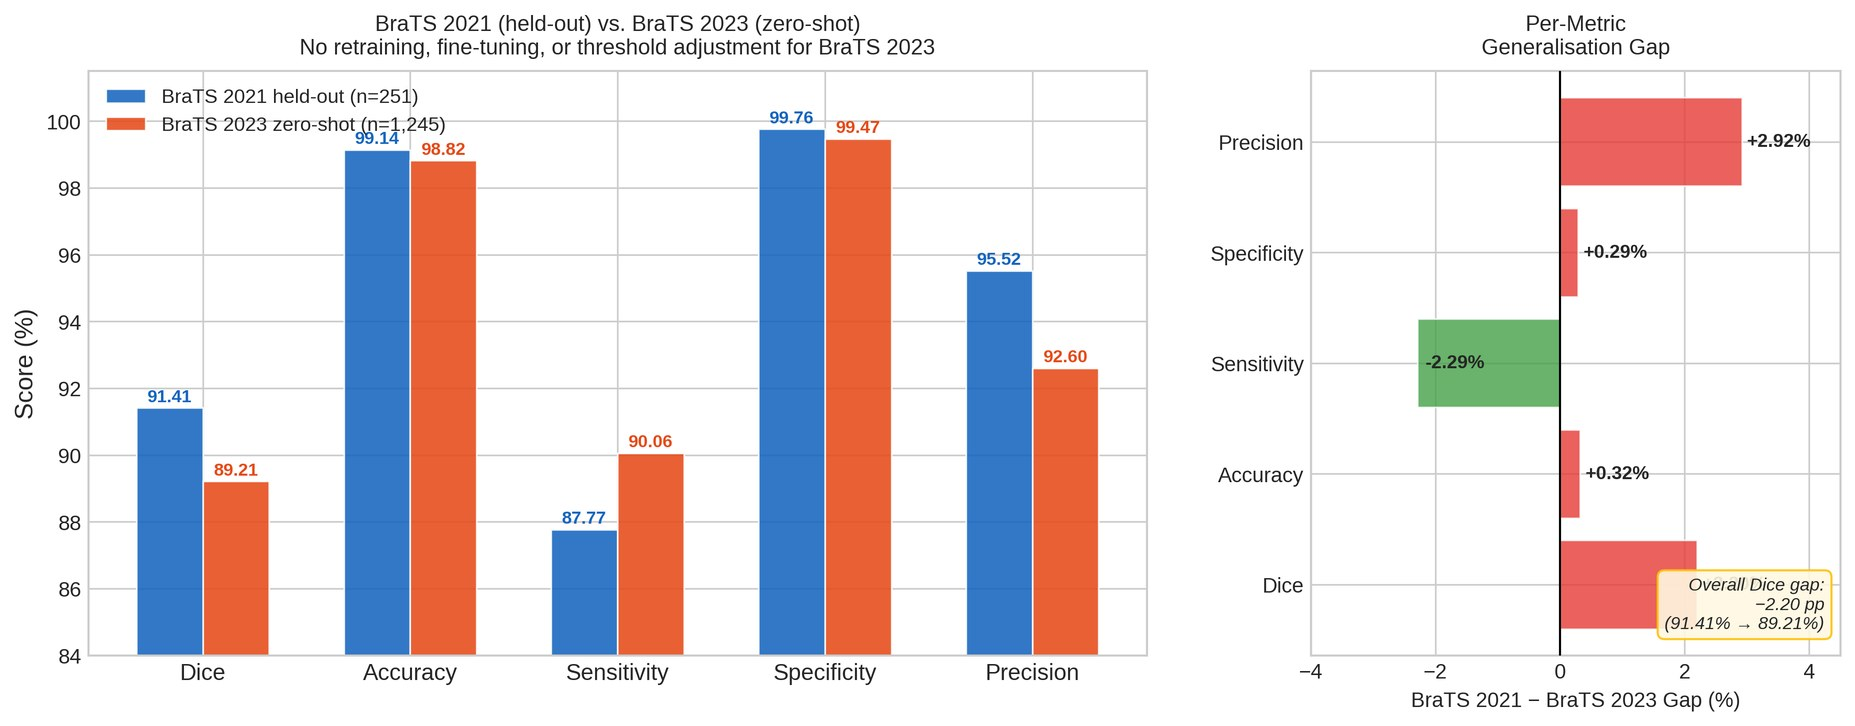
\includegraphics[width=\textwidth]{fig_C_generalisation.jpg}
\caption{\textbf{Cross-Edition Generalisation: BraTS 2021 vs.\ BraTS 2023.}
\textit{Left}: Grouped bar chart for all five metrics. \textit{Right}: Per-metric
gap (BraTS 2021 $-$ BraTS 2023). Dice drops by 2.01\,pp; sensitivity
\textit{improves} by $+$2.92\,pp, indicating tumour recall is preserved.
Precision drops 3.06\,pp, consistent with a slightly higher false-positive rate
on BraTS 2023 scanner diversity.}
\label{fig:generalisation}
\end{figure}

The ensemble achieves \textbf{89.40\%} Dice on BraTS 2023, a \textbf{2.01\,pp
generalisation gap}. A notable finding: sensitivity \textit{improves} by
$+$2.92\,pp on BraTS 2023 (87.77\%~$\rightarrow$~90.69\%), while precision drops
by 3.06\,pp. This pattern is consistent with scanner- and annotation-protocol-driven
distribution shift between challenge editions: the model over-detects slightly on
BraTS 2023, producing more true positives but also more false positives. The
elevated per-patient Dice standard deviation ($\pm$11.10\%) relative to the BraTS
2021 fold-level spread ($\pm$0.66\,pp) reflects the broader morphological and
scanner diversity of the 2023 cohort.

\subsection{Qualitative Analysis and Per-Patient Distribution}

\begin{figure}[htbp]
\centering
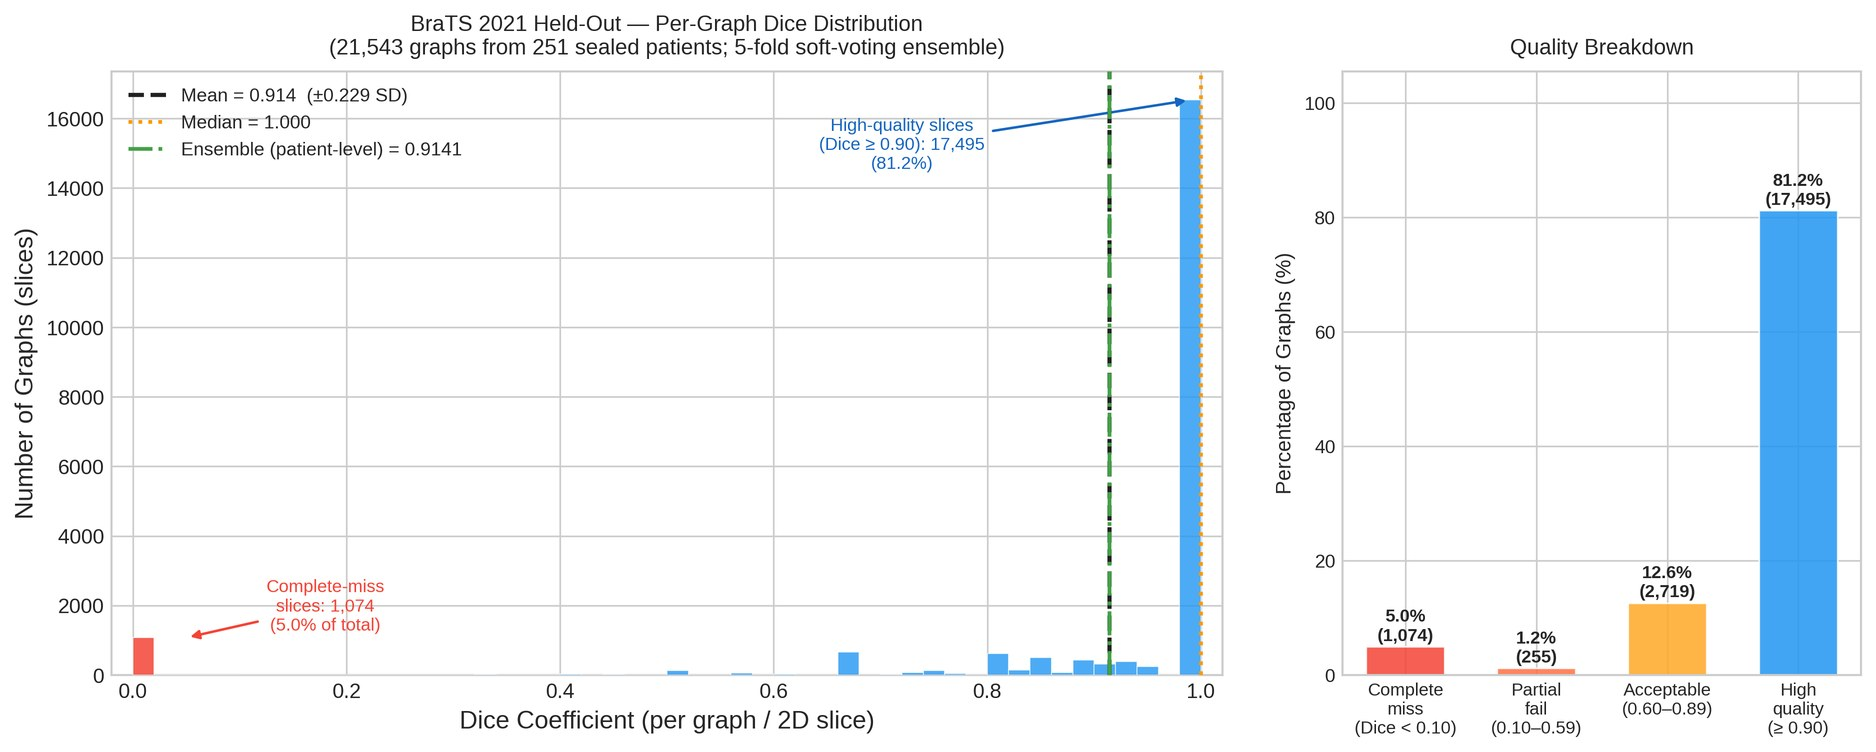
\includegraphics[width=\textwidth]{fig_G_dice_distribution.jpg}
\caption{\textbf{Per-Graph Dice Distribution --- BraTS 2021 Held-Out (251 patients).}
\textit{Left}: Per-graph Dice histogram; red bins (Dice $<$ 0.10) are complete-miss
slices (5.0\% of graphs); dominant high-quality peak (Dice $\geq$ 0.90: 81.2\%).
Dashed line: per-slice mean (83.2\%); dash-dot line: patient-level ensemble Dice
(91.41\%). \textit{Right}: Quality tier breakdown pie chart.}
\label{fig:dice_hist}
\end{figure}

\begin{figure}[htbp]
\centering
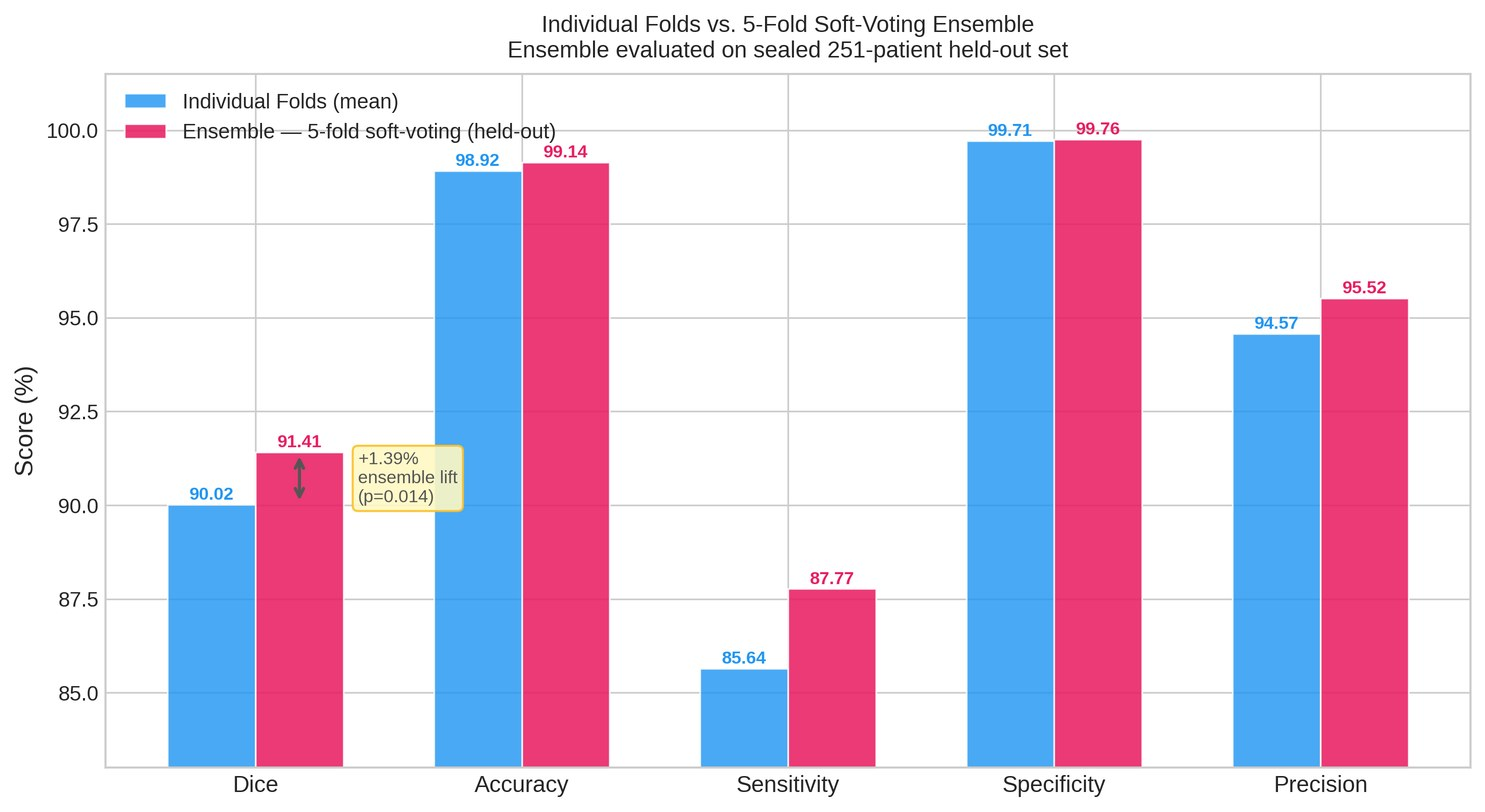
\includegraphics[width=\textwidth]{fig_E_ensemble_vs_individual.jpg}
\caption{\textbf{Ensemble vs.\ Individual Fold Models.}
Per-fold Dice on the sealed held-out set alongside the ensemble result (91.41\%).
The $+1.39$\,pp lift demonstrates the benefit of soft-voting aggregation over
any single model.}
\label{fig:ensemble}
\end{figure}

81.2\% of per-graph slices achieve Dice $\geq$ 0.90, and only 5.0\% are complete
misses (Dice $<$ 0.10). Three worst-case patients (BraTS2021\_01405, \_01366,
\_01407) received near-zero Dice scores ($\leq 5\times10^{-8}$): the model predicts
all-background on volumes with atypical or absent T1CE enhancement, where superpixel
features fail to separate tumour from background. This complete-miss failure mode is
structurally distinct from boundary imprecision (the dominant error at median
performance) and is clinically more consequential. Patient BraTS2021\_01594 achieved
perfect Dice (100\%) across 8,067 tumour superpixels, confirming that full
discrimination is achievable when T1CE contrast is strong.

% ============================================================
\section{Discussion}
\label{sec:discussion}
% ============================================================

\subsection{Efficiency as a Structural Property}

The central result is that a 439K-parameter GNN trained on sparse superpixel graphs
matches or exceeds the accuracy of a 68M-parameter U-Net trained under identical
hardware constraints, while consuming 227$\times$ less GPU memory and running
5.9$\times$ faster end-to-end. This is not a training-trick result. The efficiency
advantage is \textit{structural}: it arises from the fundamental difference between
dense 3D convolution on 8.9M voxels and message-passing on $\approx$3,909 graph
nodes per patient. The parameter reduction, memory savings, and speedup hold
regardless of how well either model is individually tuned.

Three qualifications apply to this comparison. First, the 3D U-Net baseline is
trained with binary-only labels; published multi-class U-Net results (91--92\% WT
Dice) benefit from auxiliary gradient signal across ET/TC/WT sub-regions unavailable
in the binary formulation. A fully-tuned binary U-Net on larger hardware would likely
narrow the accuracy gap to near-zero, but would not alter the structural efficiency
advantages. Second, graph construction adds $\approx$1.66\,s overhead per patient
at first build time; in clinical batch-processing workflows, pre-cached graphs reduce
this to the 75.4\,ms inference-only figure. Third, the 15 handcrafted features encode
domain knowledge that must be adapted for tumour types outside gliomas.

\subsection{The Complete-Miss Failure Mode}

5\% of per-graph slices receive near-zero Dice scores, concentrated among patients
with atypical or absent T1CE enhancement. This failure mode is qualitatively
different from boundary imprecision: the model predicts all-background, resulting
in the patient being missed entirely rather than partially segmented. \textbf{Any
clinical deployment must include a post-processing gate that detects all-zero
output masks and flags them for mandatory radiologist review.} Addressing the root
cause requires adaptive superpixel granularity (finer regions near low-contrast
tumour boundaries), augmentation of atypical enhancement cases during training, or
learned feature representations that do not depend on strong T1CE contrast as the
primary discriminative signal.

\subsection{Comparison with State-of-the-Art}

Table~\ref{tab:sota} contextualises our results. Our binary ensemble (91.41\%) is
within 1.3--1.9\,pp of leading multi-class transformer methods that solve the harder
three-class problem with auxiliary supervision and $\geq$14$\times$ more parameters.
On the directly comparable binary task under the same hardware constraints, our GNN
achieves $+$3.91\,pp over the constrained U-Net baseline.

\begin{table}[htbp]
\caption{Context vs.\ Published Methods on BraTS 2021 WT Dice}
\begin{center}
\begin{tabularx}{\textwidth}{|>{\raggedright\arraybackslash}X
  |>{\centering\arraybackslash}X|>{\centering\arraybackslash}X|>{\centering\arraybackslash}X|}
\hline
\textbf{Method} & \textbf{WT Dice (\%)} & \textbf{Params} & \textbf{Task}\\
\hline
3D U-Net \cite{cicek20163d} & 91.2 & 68M & Multi-class\\
\hline
nnU-Net \cite{isensee2021nnunet} & $\sim$92.7 & 31M & Multi-class\\
\hline
TransBTS \cite{wang2021transbts} & 90.1 & 33M & Multi-class\\
\hline
Swin-UNETR \cite{hatamizadeh2022swin} & 93.3 & 62M & Multi-class\\
\hline
\hline
3D U-Net (binary, our replica)$^\dagger$ & 87.5 & 68M & Binary\\
\hline
\textbf{GraphSAGE 5L (ours)}$^\dagger$ & \textbf{90.02$\pm$0.66} & \textbf{439K} & Binary\\
\hline
\textbf{GraphSAGE Ensemble (ours)}$^\dagger$ & \textbf{91.41} & \textbf{2.2M} & Binary\\
\hline
\end{tabularx}
\end{center}
\label{tab:sota}
{\footnotesize $^\dagger$ Measured on RTX 2060, 6\,GB VRAM. Multi-class methods
benefit from ET/TC auxiliary supervision unavailable in binary training; their WT
Dice is provided as scale reference only, not as a direct comparison. Comparing
multi-class WT Dice with binary WT Dice systematically disadvantages our method
and is acknowledged as a limitation.}
\end{table}

\subsection{Deployment Implications}

The 75.4\,ms (pre-built graph) / 1.73\,s (end-to-end) inference times, 11\,MB peak
GPU memory, and 1.7\,MB model weight file collectively enable deployment scenarios
that are structurally infeasible for volumetric methods:
\begin{itemize}
    \item \textbf{Consumer-grade hardware.} Accurate inference on an RTX 2060
    (\$300--400) removes the hardware barrier for clinics in low- and middle-income
    countries that cannot procure A100-class GPUs (\$10,000+).
    \item \textbf{Edge and embedded deployment.} A 1.7\,MB model can be loaded onto
    embedded inference hardware for point-of-care or telemedicine devices.
    \item \textbf{High-throughput screening.} 11\,MB peak memory allows multiple
    concurrent inference processes on the same 6\,GB VRAM device, enabling batch
    screening workflows.
    \item \textbf{Interactive clinical use.} 75.4\,ms per-patient inference with
    pre-built graphs enables real-time feedback within a radiologist's review session.
\end{itemize}

% ============================================================
\section{Conclusion}
\label{sec:conclusion}
% ============================================================

We presented a superpixel-graph formulation for binary brain tumour segmentation
that achieves \textbf{91.41\% ensemble Dice} on a sealed 251-patient BraTS 2021
held-out set with \textbf{439,041 parameters}, \textbf{75.4\,ms} per-patient GNN
inference, and \textbf{11\,MB} peak GPU memory. Five-fold cross-validation confirms
\textbf{90.02\%\,$\pm$\,0.66\%} Dice with a 1.76\,pp inter-fold range. Zero-shot
transfer to BraTS 2023 yields \textbf{89.40\%} Dice (2.01\,pp gap, 1,245 patients),
demonstrating cross-edition robustness without any retraining. End-to-end processing
per patient requires \textbf{1,732\,ms} including on-the-fly SLIC graph construction,
a \textbf{5.9$\times$ speedup} over a hardware-matched 3D U-Net; for pre-cached
graphs, GNN inference takes \textbf{75.4\,ms}.

Systematic ablation on Fold 0 confirms the 5-layer, 256-dim GraphSAGE configuration
as Pareto-optimal under a 6\,GB VRAM constraint: added depth provides no accuracy
benefit, while the wider 512-dim and attention-based GAT variants trade efficiency
for modest gains at unacceptably higher parameter cost under this constraint. The
dominant failure mode---complete-miss predictions on patients with atypical T1CE
enhancement---is characterised, and a mandatory empty-prediction detection gate is
specified as a prerequisite for any clinical deployment.

These results demonstrate that graph-structured representations constitute a
practically deployable alternative to volumetric convolution for brain tumour
detection, enabling AI-assisted diagnostics on consumer-grade hardware where
3D CNN-based pipelines are not feasible.

\textbf{Limitations.}
This work addresses binary whole-tumour segmentation only; the 1.3--1.9\,pp gap
from multi-class SOTA methods (nnU-Net, Swin-UNETR) is partially attributable to
the absence of auxiliary ET/TC gradient signal. Cross-dataset evaluation is limited
to BraTS 2021$\rightarrow$2023; performance on non-glioma tumour types (meningioma,
metastases) and post-treatment imaging is untested. The 15 handcrafted node features
require domain expertise and may not generalise without modification to other tumour
types or scanner protocols.

\textbf{Future work.}
Immediate priorities: (1) multi-task extension for simultaneous ET/TC/WT prediction;
(2) GPU-accelerated SLIC to reduce end-to-end latency below 100\,ms; (3) adaptive
superpixel granularity to address complete-miss failures on low-contrast lesions;
and (4) prospective radiologist evaluation studies as a prerequisite for regulatory
pathway consideration.

% ============================================================
%  BIBLIOGRAPHY
% ============================================================
\cleardoublepage
\bibliographystyle{unsrtnat}
\bibliography{ref.bib}

\end{document}
